

\tikzset{every picture/.style={line width=0.75pt}} %set default line width to 0.75pt        

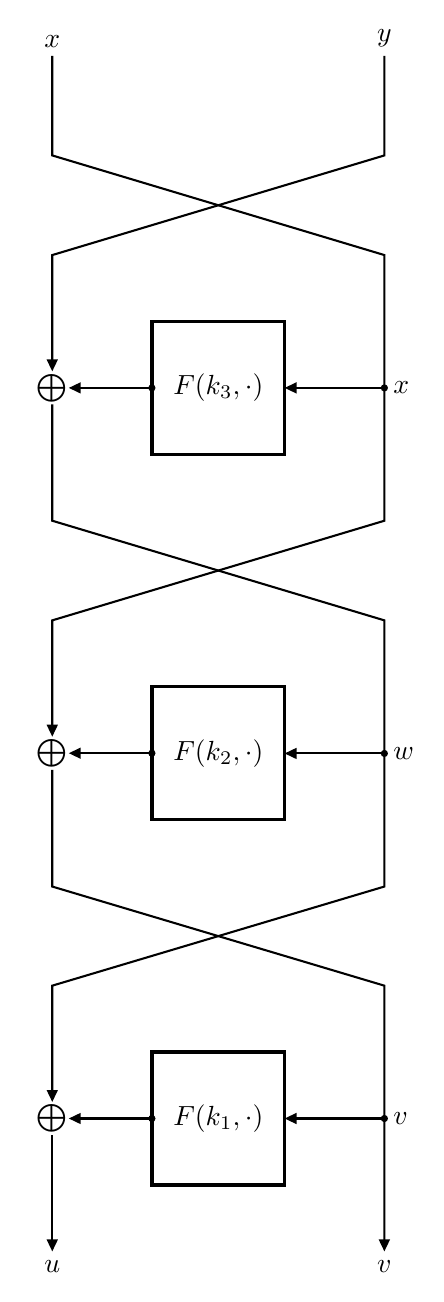
\begin{tikzpicture}[x=0.75pt,y=0.75pt,yscale=-0.8,xscale=0.8]
%uncomment if require: \path (0,809); %set diagram left start at 0, and has height of 809

%Shape: Rectangle [id:dp08810068320716669] 
\draw  [line width=1.2]  (80,200) -- (160,200) -- (160,280) -- (80,280) -- cycle ;
%Straight Lines [id:da7148920386750357] 
\draw    (20,249.96) -- (20,320) -- (220,380) -- (220,540.31) -- (20,600) -- (20,667) ;
\draw [shift={(20,670)}, rotate = 270] [fill={rgb, 255:red, 0; green, 0; blue, 0 }  ][line width=0.08]  [draw opacity=0] (7.14,-3.43) -- (0,0) -- (7.14,3.43) -- cycle    ;
%Shape: Rectangle [id:dp05753096156132376] 
\draw  [line width=1.2]  (80,420) -- (160,420) -- (160,500) -- (80,500) -- cycle ;
%Shape: Rectangle [id:dp5426589489554612] 
\draw  [line width=1.2]  (80,640) -- (160,640) -- (160,720) -- (80,720) -- cycle ;
%Straight Lines [id:da36785755794381103] 
\draw    (20,40) -- (20,100) -- (220,160) -- (220,320) -- (20,380) -- (20,447) ;
\draw [shift={(20,450)}, rotate = 270] [fill={rgb, 255:red, 0; green, 0; blue, 0 }  ][line width=0.08]  [draw opacity=0] (7.14,-3.43) -- (0,0) -- (7.14,3.43) -- cycle    ;
%Straight Lines [id:da5270839120181066] 
\draw    (220,40) -- (220,100) -- (20,160) -- (20,227) ;
\draw [shift={(20,230)}, rotate = 270] [fill={rgb, 255:red, 0; green, 0; blue, 0 }  ][line width=0.08]  [draw opacity=0] (7.14,-3.43) -- (0,0) -- (7.14,3.43) -- cycle    ;
%Straight Lines [id:da30154795477439555] 
\draw    (20,690) -- (20,757) ;
\draw [shift={(20,760)}, rotate = 270] [fill={rgb, 255:red, 0; green, 0; blue, 0 }  ][line width=0.08]  [draw opacity=0] (7.14,-3.43) -- (0,0) -- (7.14,3.43) -- cycle    ;
%Straight Lines [id:da9103919429832117] 
\draw    (20,470) -- (20,540.31) -- (220,600) -- (220,757) ;
\draw [shift={(220,760)}, rotate = 270] [fill={rgb, 255:red, 0; green, 0; blue, 0 }  ][line width=0.08]  [draw opacity=0] (7.14,-3.43) -- (0,0) -- (7.14,3.43) -- cycle    ;
%Straight Lines [id:da3209792329411032] 
\draw    (220,240) -- (163,240) ;
\draw [shift={(160,240)}, rotate = 360] [fill={rgb, 255:red, 0; green, 0; blue, 0 }  ][line width=0.08]  [draw opacity=0] (7.14,-3.43) -- (0,0) -- (7.14,3.43) -- cycle    ;
%Straight Lines [id:da07595236987438247] 
\draw    (80,240) -- (33,240) ;
\draw [shift={(30,240)}, rotate = 360] [fill={rgb, 255:red, 0; green, 0; blue, 0 }  ][line width=0.08]  [draw opacity=0] (7.14,-3.43) -- (0,0) -- (7.14,3.43) -- cycle    ;
%Straight Lines [id:da8515371795008031] 
\draw    (220,460.15) -- (163,460.15) ;
\draw [shift={(160,460.15)}, rotate = 360] [fill={rgb, 255:red, 0; green, 0; blue, 0 }  ][line width=0.08]  [draw opacity=0] (7.14,-3.43) -- (0,0) -- (7.14,3.43) -- cycle    ;
%Straight Lines [id:da08233223837321657] 
\draw    (220,680) -- (163,680) ;
\draw [shift={(160,680)}, rotate = 360] [fill={rgb, 255:red, 0; green, 0; blue, 0 }  ][line width=0.08]  [draw opacity=0] (7.14,-3.43) -- (0,0) -- (7.14,3.43) -- cycle    ;
%Straight Lines [id:da3216064715402762] 
\draw    (80,460) -- (33,460) ;
\draw [shift={(30,460)}, rotate = 360] [fill={rgb, 255:red, 0; green, 0; blue, 0 }  ][line width=0.08]  [draw opacity=0] (7.14,-3.43) -- (0,0) -- (7.14,3.43) -- cycle    ;
%Straight Lines [id:da0911188498517359] 
\draw    (80,680) -- (33,680) ;
\draw [shift={(30,680)}, rotate = 360] [fill={rgb, 255:red, 0; green, 0; blue, 0 }  ][line width=0.08]  [draw opacity=0] (7.14,-3.43) -- (0,0) -- (7.14,3.43) -- cycle    ;
%Shape: Circle [id:dp5566373818887096] 
\draw  [fill={rgb, 255:red, 0; green, 0; blue, 0 }  ,fill opacity=1 ] (218.5,240) .. controls (218.5,239.17) and (219.17,238.5) .. (220,238.5) .. controls (220.83,238.5) and (221.5,239.17) .. (221.5,240) .. controls (221.5,240.83) and (220.83,241.5) .. (220,241.5) .. controls (219.17,241.5) and (218.5,240.83) .. (218.5,240) -- cycle ;
%Shape: Circle [id:dp14089569320942252] 
\draw  [fill={rgb, 255:red, 0; green, 0; blue, 0 }  ,fill opacity=1 ] (78.5,240) .. controls (78.5,239.17) and (79.17,238.5) .. (80,238.5) .. controls (80.83,238.5) and (81.5,239.17) .. (81.5,240) .. controls (81.5,240.83) and (80.83,241.5) .. (80,241.5) .. controls (79.17,241.5) and (78.5,240.83) .. (78.5,240) -- cycle ;
%Shape: Circle [id:dp9889295507534646] 
\draw  [fill={rgb, 255:red, 0; green, 0; blue, 0 }  ,fill opacity=1 ] (78.5,460) .. controls (78.5,459.17) and (79.17,458.5) .. (80,458.5) .. controls (80.83,458.5) and (81.5,459.17) .. (81.5,460) .. controls (81.5,460.83) and (80.83,461.5) .. (80,461.5) .. controls (79.17,461.5) and (78.5,460.83) .. (78.5,460) -- cycle ;
%Shape: Circle [id:dp6544997090075493] 
\draw  [fill={rgb, 255:red, 0; green, 0; blue, 0 }  ,fill opacity=1 ] (218.5,460.15) .. controls (218.5,459.33) and (219.17,458.65) .. (220,458.65) .. controls (220.83,458.65) and (221.5,459.33) .. (221.5,460.15) .. controls (221.5,460.98) and (220.83,461.65) .. (220,461.65) .. controls (219.17,461.65) and (218.5,460.98) .. (218.5,460.15) -- cycle ;
%Shape: Circle [id:dp16907136977415704] 
\draw  [fill={rgb, 255:red, 0; green, 0; blue, 0 }  ,fill opacity=1 ] (218.5,680) .. controls (218.5,679.17) and (219.17,678.5) .. (220,678.5) .. controls (220.83,678.5) and (221.5,679.17) .. (221.5,680) .. controls (221.5,680.83) and (220.83,681.5) .. (220,681.5) .. controls (219.17,681.5) and (218.5,680.83) .. (218.5,680) -- cycle ;
%Shape: Circle [id:dp3827346476021749] 
\draw  [fill={rgb, 255:red, 0; green, 0; blue, 0 }  ,fill opacity=1 ] (78.5,680) .. controls (78.5,679.17) and (79.17,678.5) .. (80,678.5) .. controls (80.83,678.5) and (81.5,679.17) .. (81.5,680) .. controls (81.5,680.83) and (80.83,681.5) .. (80,681.5) .. controls (79.17,681.5) and (78.5,680.83) .. (78.5,680) -- cycle ;

% Text Node
\draw (20,240) node   {$\bigoplus $};
% Text Node
\draw (20,460) node   {$\bigoplus $};
% Text Node
\draw (20,680) node   {$\bigoplus $};
% Text Node
\draw (120,240) node    {$F( k_{3} ,\cdot )$};
% Text Node
\draw (120,460) node    {$F( k_{2} ,\cdot )$};
% Text Node
\draw (120,680) node    {$F( k_{1} ,\cdot )$};
% Text Node
\draw (20,36.6) node [anchor=south] [inner sep=0.75pt]    {$x$};
% Text Node
\draw (220,36.6) node [anchor=south] [inner sep=0.75pt]    {$y$};
% Text Node
\draw (223.5,240) node [anchor=west] [inner sep=0.75pt]    {$x$};
% Text Node
\draw (223.5,460.15) node [anchor=west] [inner sep=0.75pt]    {$w$};
% Text Node
\draw (223.5,680) node [anchor=west] [inner sep=0.75pt]    {$v$};
% Text Node
\draw (220,763.4) node [anchor=north] [inner sep=0.75pt]    {$v$};
% Text Node
\draw (20,763.4) node [anchor=north] [inner sep=0.75pt]    {$u$};


\end{tikzpicture}